%% --------------------------------------------------------------------------
% LaTeX template for the XLIV CILAMCE
%
% This latex document tries to copy the Microsoft Word template.
% --------------------------------------------------------------------------
\documentclass[a4paper,10pt]{book}

% PACKAGES USED - packages that need to be previously installed on your computer
\usepackage[lmargin=2.5cm, rmargin=2.5cm, tmargin=2.5cm, bmargin=2.5cm ]{geometry}
\usepackage{graphicx}
\usepackage{times}
\usepackage{indentfirst}
\usepackage{fancyhdr}
\usepackage{titlesec}
\usepackage[english]{babel}
\usepackage{parskip} 
\usepackage{setspace}

%Package to hold figure in position
\usepackage{placeins}


% Mathematical Symbols
\newcommand{\dgds}{\boldsymbol{g_\sigma}}
\newcommand{\Dll}{\boldsymbol{D}}
\newcommand{\Dllmod}{\boldsymbol{D^{*}}}
\newcommand{\Dllepvp}{\boldsymbol{D}^{epvp}}
\newcommand{\dstrain}{\boldsymbol{\dot{\varepsilon}}}
\newcommand{\dstraine}{\boldsymbol{\dot{\varepsilon}}^{e}}
\newcommand{\dstrainp}{\boldsymbol{\dot{\varepsilon}}^{p}}
\newcommand{\dstrainv}{\boldsymbol{\dot{\varepsilon}}^{vp}}
\newcommand{\straineqp}{\bar \varepsilon^p}
\newcommand{\dstrainsh}{\boldsymbol{\dot{\varepsilon}}^{sh}}
\newcommand{\dstraincr}{\boldsymbol{\dot{\varepsilon}}^{cr}}
\newcommand{\dstress}{\boldsymbol{\dot{\sigma}}}

\newcommand{\ex}{\boldsymbol{e}_x}
\newcommand{\ey}{\boldsymbol{e}_y}
\newcommand{\ez}{\boldsymbol{e}_z}

\newcommand{\onell}{\boldsymbol{1}}
\newcommand{\strain}{\boldsymbol{\varepsilon}}
\newcommand{\straincr}{\boldsymbol{\varepsilon}^{cr}}
\newcommand{\straine}{\boldsymbol{\varepsilon}^{e}}
\newcommand{\strainp}{\boldsymbol{\varepsilon}^{p}}
\newcommand{\strainsh}{\boldsymbol{\varepsilon}^{sh}}
\newcommand{\strainshCEB}{\varepsilon_{sh}}
\newcommand{\strainvp}{\boldsymbol{\varepsilon}^{vp}}
\newcommand{\stress}{\boldsymbol{\sigma}}
\newcommand{\zerol}{\boldsymbol 0}

%%%%%%%%%%%%%%%%%%%%%%%%%%%%%%%%%%%%%%%%%%%%%%%%%%%%%%%%%%%%%%%%%
%%%%%%%%%%%%%%%%%%%%%%%%%%%%%%%%%%%%%%%%%%%%%%%%%%%%%%%%%%%%%%%%%
%%% My Additional Packages
%%%%%%%%%%%%%%%%%%%%%%%%%%%%%%%%%%%%%%%%%%%%%%%%%%%%%%%%%%%%%%%%%
\usepackage[utf8]{inputenc}
\usepackage{amssymb} %Mathematics
\usepackage{amsfonts}%Mathematics
\usepackage{amsmath,amscd}%Mathematics
\usepackage{amsthm}%Mathematics
\usepackage{mathrsfs}%Mathematics font
\usepackage{xspace}
\usepackage{booktabs}
\usepackage{stmaryrd}%Particular Brackets
\usepackage{graphicx} %Tables and Figures
\usepackage{subfigure}
\usepackage{url}
\usepackage{hyperref}
\usepackage{cleveref}
\usepackage{./pkg-crefNames}
\usepackage[labelsep=period]{caption}
%\usepackage{mathptmx}
\usepackage{newtxtext,newtxmath}
\usepackage{bm}

\hypersetup{hidelinks}

%BibTeX compatible with the CILAMCE format
\usepackage[numbers,sort&compress]{natbib}

\setlength{\bibsep}{0pt plus 0.3ex}

\renewcommand*{\bibfont}{\small}

\makeatletter
\renewcommand\bibsection
{
  \section*{References}
}



\renewenvironment{thebibliography}[1]
      {\section*{\refname}%
       \@mkboth{\MakeUppercase\refname}{\MakeUppercase\refname}%
       \list{\@biblabel{\@arabic\c@enumiv}}%
            {\settowidth\labelwidth{\@biblabel{#1}}%
             \leftmargin\labelwidth
             \advance\leftmargin-10pt% change 20 pt according to your needs
             \advance\leftmargin\labelsep
             \setlength\itemindent{10pt}% change using the inverse of the length used before
             \@openbib@code
             \usecounter{enumiv}%
             \let\p@enumiv\@empty
             \renewcommand\theenumiv{\@arabic\c@enumiv}}%
       \sloppy
       \clubpenalty4000
       \@clubpenalty \clubpenalty
       \widowpenalty4000%
       \sfcode`\.\@m}
      {\def\@noitemerr
        {\@latex@warning{Empty `thebibliography' environment}}%
       \endlist}
\renewcommand\newblock{\hskip .11em\@plus.33em\@minus.07em}
\makeatother




\makeatother
\bibliographystyle{./bib-cilamce}
%\bibliographystyle{plain}


%%%%%%%%%%%%%%%%%%%%%%%%%%%%%%%%%%%%%%%%%%%%%%%%%%%%%%%%%%%%%%%%%
%%%%%%%%%%%%%%%%%%%%%%%%%%%%%%%%%%%%%%%%%%%%%%%%%%%%%%%%%%%%%%%%%

% CONFIGURATION
\renewcommand*\arraystretch{1.5}
\renewcommand*\thesection{\arabic{section}}
%\hyphenpenalty=10000 % You can uncomment this to avoid hyphenization
\titleformat*{\section}{\large\bfseries}
\titleformat*{\subsection}{\bfseries}
\titlespacing\section{0pt}{20pt plus 2pt minus 2pt}{12pt plus 2pt minus 2pt}
\titlespacing\subsection{0pt}{20pt plus 0pt minus 0pt}{12pt plus 0pt minus 0pt}
\setlength{\parskip}{0pt} % Spacing between paragraphs
\setlength{\parindent}{0.75cm} % Paragraph identation
\setlength\abovecaptionskip{6pt}

% --------------------------------------------------------------------------
% DO NOT EDIT - SPECIAL HEADINGS OF XLIII CILAMCE
% --------------------------------------------------------------------------
\fancypagestyle{first}
{
\fancyhf{}
\fancyfoot[RO]{\footnotesize \textit{CILAMCE-2024 \\
Proceedings of the XLV Ibero-Latin-American Congress on Computational Methods in Engineering, ABMEC\\
Maceió, Alagoas, November 11-14, 2024}}
\renewcommand{\headrulewidth}{.0pt}
\renewcommand{\footrulewidth}{.5pt}
}

\pagestyle{fancy}
\fancyhf{}

\fancyfoot[LE]{\footnotesize \textit{CILAMCE-2024\\
Proceedings of the XLV Ibero-Latin-American Congress on Computational Methods in Engineering, ABMEC\\
Maceió, Alagoas, November 11-14, 2024}}

\fancyfoot[RO]{\footnotesize \textit{CILAMCE-2024\\
Proceedings of the XLV Ibero-Latin-American Congress on Computational Methods in Engineering, ABMEC\\
Maceió, Alagoas, November 11-14, 2024}}




\renewcommand{\headrulewidth}{.5pt}
\renewcommand{\footrulewidth}{.5pt}

% --------------------------------------------------------------------------
% PLEASE, EDIT THIS!
\fancyhead[LE]{\footnotesize \textit{Finite Element Analysis of Rock Deformation in Deep Twin Tunnels}}
\fancyhead[RO]{\footnotesize \textit{Felipe P. M. Quevedo, Carlos A. M. M. Colombo, Bianca M. Girardi, Denise Bernaud, Samir Maghous}}
% --------------------------------------------------------------------------

\begin{document}\thispagestyle{first}

% --------------------------------------------------------------------------
% DO NOT EDIT - LOGO OF XLIII CILAMCE
% --------------------------------------------------------------------------

\begin{figure}[ht!]
\vspace{-30pt}
\flushright

\includegraphics[width=4.3cm]{Figures/logo.png}
%scale=0.25
\end{figure}

% --------------------------------------------------------------------------
% TITLE OF PAPER
% --------------------------------------------------------------------------

\noindent
\textbf{\Large
Finite Element Analysis of Rock Deformation in Deep Twin Tunnels} 
\vspace{18pt} % <- keep this vertical space!

% --------------------------------------------------------------------------
% AUTHORS
% --------------------------------------------------------------------------

\noindent Felipe P. M. Quevedo$^1$, Carlos A. M. M. Colombo$^1$, Bianca M. Girardi$^1$, Denise Bernaud$^1$, Samir Maghous$^1$

\vspace{18pt} % <- keep this vertical space!

\noindent $^1$\textit{Graduate Program in Civil Engineering, Federal University of Rio Grande do Sul}

\noindent \textit{Av. Osvaldo Aranha, 99, Porto Alegre, 90.035-190, RS, Brazil}

\noindent \textit{motta.quevedo@ufrgs.br, ca-colombo@hotmail.com, eng.biancagirardi@gmail.com}

\noindent \textit{denise.bernaud@ufrgs.br, samir.maghous@ufrgs.br}


\vspace{18pt} % <- keep this vertical space!

% --------------------------------------------------------------------------
% ABSTRACT
% --------------------------------------------------------------------------

\noindent \textbf{Abstract.}
Relying upon a three-dimensional finite element analysis, this contribution investigates the instantaneous irreversible response induced by the constitutive behavior of the rock mass in the convergence profile of twin tunnels with transverse gallery. At the rock material level, elastoplastic state equations based on a Drucker-Prager yield surface with an associated flow rule are adopted in the modeling. As regards the tunnel support, the formulation accounts for the presence of an elastic shotcrete-like lining. From a computational point of view, the deactivation-activation method is used to simulate the excavation process and the installation of the lining. The accuracy of the finite element predictions is assessed through comparisons with the available analytical solutions formulated in a simplified scenario for the twin tunnel configuration. A parametric study investigates the mutual interaction induced by the proximity of the tunnels and the influence of the lining stiffness.

\vspace{18pt} % <- keep this vertical space!

\noindent \textbf{Keywords:} Twin tunnels, Transverse gallery, Elastoplasticity, Finite element modeling


% --------------------------------------------------------------------------
\section{Introduction}\label{sec:introduction}
% --------------------------------------------------------------------------
Many design methods often focus on single tunnels, however twin tunnels are a common occurrence. The interaction between tunnels can be significant, especially when the spacing between them is minimal. Additionally, many twin tunnels incorporate transverse galleries, introducing a localized effect on displacements and stresses. While the simulation of tunnel convergence in single tunnels has been widely investigated and reported in published
literature, few works have addressed the computational evaluation of deformation in twin tunnels. Some studies on deep twin tunnels can be found at \citet{Spyridis2015}, \citet{Chen2019}, \citet{MA2020}, \citet{Fortsakis2021}, \citet{chortis2021a}, \citet{chortis2021b}, \citet{GUO2021}, \citet{chortis2023a}, \citet{chortis2023b}. However, less attention has been dedicated to assessing the mutual mechanical interaction induced by the excavation of the transverse gallery connecting the twin tunnels.

In this context, the main contributions of this paper can be summarized at both the material and tunnel analysis levels. At the material level, the constitutive state equations of the rock mass are developed using a plasticity framework, which is suitable for clayey rocks. For the mechanical behavior of the concrete lining, the traditional linear elastic model is employed. At the structural analysis level, the deformation of the highly interactive components of the material system (i.e., rock mass and lining) resulting from the excavation of twin tunnels and transverse gallery is simulated using three-dimensional finite element simulations. The excavation and lining placement processes are simulated through the activation/deactivation technique. The constitutive models for the rock mass and the associated numerical integration schemes are implemented into the UPF/USERMAT customization tool [\citenum{ANSYS:2013b}] of the ANSYS standard software. This three-dimensional finite element analysis is specifically designed to address the interactions induced by the construction process, the proximity of twin tunnels, and the presence of the transverse gallery.

% --------------------------------------------------------------------------
\section{Constitutive Models}\label{sec:format}
% --------------------------------------------------------------------------

The constitutive model for the rock mass corresponds to the associated Drucker-Prager elastoplastic model. The local strain rate $\dstrain$ is split into two contributions $\dstrain = \dstraine + \dstrainp$, so that the constitutive relationships relating the Cauchy stress rate $\dstress$ and strain rate components can be written as:
\begin{equation} \label{eq_constitutive_relationship_epvp}
	\dstress = \Dll : \dstraine = \Dll : (\dstrain - \dstrainp)\;
\end{equation}

In the above relationship, $\dstraine$ and $\dstrainp$, represent respectively the elastic and plastic strain rate, and $\Dll$ denote the fourth-order isotropic elastic linear constitutive tensor defined by the rock mass elastic Young modulus $E$ and Poisson ratio $\nu$. The plastic strain rate is given by the flow rule:
\begin{equation}
	\label{eq_plastic_flow}
	\dot \strainp = \left\{ 
	\begin{array}{ll} 
		\dot \lambda \dfrac{\partial g}{\partial \stress} &  \text{for } f > 0 \\ 
		\zerol, & \text{for } f \le 0 \\
	\end{array}\right.
\end{equation}
where $\dot \lambda$ is the plasticity multiplier (obtained through the consistency condition  $\dot f = 0$) and $g$ is a potential flow function analogous to $f$ used to simulate the volume dilatation during the evolution of plastic deformations. However, for this analysis, associated plasticity was adopted, i.e., $g=f$. In this model, the Drucker-Prager plastic flow surface is given by
\begin{equation}
	\label{eq:f_Drucker_Prager}
	f(\stress,q) = f(I_1,J_2,q) = \beta_1 I_1 +\beta_2 \sqrt{J_2}-q(\alpha)
\end{equation}
which $I_1$ is the first invariant of the stress tensor, $J_2$ is the second invariant of the deviator tensor and $\beta_1, \beta_2$ and $q(\alpha)$ are strength parameters related to the friction angle $\phi$ and cohesion $c(\alpha)$, respectively. The Drucker-Prager plasticity surface inscribed in the Mohr-Coulomb surface is considered, i.e. [\citenum{bernaud1991}]:
\begin{equation}
	\label{eq:f_DP_inscrita_MC}
	\beta_1 = \dfrac{(k-1)}{3}, ~~~ \beta_2 = \dfrac{(2k+1)}{\sqrt{3}}, ~~~
	q(\alpha) = 2\sqrt{k}~c(\alpha)
\end{equation}
where $k = (1+\sin{\phi})/(1-\sin{\phi})$. The internal variable $\alpha$ is the equivalent plastic strain $\straineqp$ used to simulate strain hardening/softening phenomena. However, for this study, we adopt perfect plasticity, meaning that c is a constant. 

A linear elastic constitutive model is used for the concrete lining, which can be expressed, within the framework of infinitesimal analysis, as $\dstress = \Dll : \dstraine$, where, $\dstraine$ and $\Dll$ are respectively the elastic strain rate and the fourth-order isotropic elastic constitutive tensor defined by the concrete lining Poisson ratio $\nu_c$ and elastic Young modulus $E_c$. In the analyses, for comparisons, the tunnel stiffness will be given by the following expression [\citenum{Panet1995}]:

\begin{equation} \label{eq:8}
	K_c = \frac{E_c}{1+\nu_c}\frac{R_t^2-(R_t-e_t)^2}{(1-2\nu_c)R_t+(R_t-e_t)^2}
\end{equation}
where $R_t$ is the tunnel radius and $e_t$ is the tunnel wall thickness.


% --------------------------------------------------------------------------
\section{Spatial discretization of the domain}\label{sec:format}
% --------------------------------------------------------------------------

The material domain $\Omega$ for finite element simulations is defined as a parallelepiped with dimensions $\left(L_1+L_2 \right ) \times L_3 \times d_3$ (see \cref{Mesh1}). Due to symmetry, only the material portion in the region $\left\{x \le 0, y \ge 0\right\}$ is discretized for F.E. analysis. In \cref{Mesh1}, $d_1$ represents the distance between the axes of longitudinal tunnels, $L_2$ is the total excavated length along longitudinal direction $\ez$, $d_3$ is the domain thickness along vertical direction $\ey$, $L_1$ is the length of the unexcavated region after tunneling,  $L_3$ is the domain length along transversal direction $\ex$, and $d_2$ indicates the position of the transverse gallery axis that intersects the longitudinal tunnel at $z = L_1+d_2$.

The mesh used consists of either $119740$ or $221104$ total elements (hexahedra and tetrahedra), depending on the longitudinal tunnel spacing $d_1$. To enhance model accuracy in the intersection zone, 10-node quadratic tetrahedral elements are used around the transverse gallery, while 8-node trilinear hexahedral elements are employed in the rest of the domain. Regions significantly influenced by tunneling are highlighted in light gray in \cref{Mesh1}. Two values of $d_1$ are considered in the parametric simulations: $d_1 = 16R_t$ and $4R_t$.

The concrete lining along the gallery wall, shown in red in \cref{Mesh1}, has a thickness $e_g$. The gallery radius $R_g$ is fixed at $2/3R_t$ for simplicity, with the same lining system (same concrete material and layer thickness) applied to both longitudinal tunnels. Parameters $d_5$ and $d_1$ define the size of the transition region involving tetrahedral elements in the $yz$ plane around the gallery.

The initial stress state prevailing in the rock mass prior to the tunnel excavation process is defined by constant vertical and horizontal geostatic stress $\sigma_v$ and $\sigma_h$ taking the following form:

%The geometry material domain $\Omega$ considered for the finite element simulations is defined by a parallelepiped volume of dimensions $\left(L_1+L_2 \right ) \times L_3 \times d_3$ (\cref{Mesh1}). Owing to the symmetry of the problem, only the material portion $\left\{x \le 0, y \ge 0\right\}$ is considered for F.E discretization and analysis. Referring to the notations of \cref{Mesh1}, $d_1$ is the distance between the axes of longitudinal tunnels, $L_2$  represents the total length along longitudinal direction $\ez$ of the cylindrical volume to be excavated that is considered in the numerical simulation, $d_3$ is the thickness along vertical direction $\ey$ of material domain $\Omega$, $L_1$ stands for the length of unexcavated region after total excavation process, $L_3$ is the total length along transversal direction $\ex$ of discretized material domain, $d_2$ characterizes the location of the circular transverse axis gallery that intersects the longitudinal tunnel at $z = L_1+d_2$. The length of the excavation step adopted will be denoted by $L_{pt}$. The mesh used in the simulations consists of $119740$ or $221104$ total elements (hexahedra and tetrahedra), depending on the value of spacing between longitudinal tunnels. To increase the accuracy of the model predictions in the intersection zone, the region surrounding the transverse gallery (including part of the longitudinal tunnel) is discretized by means of 10-node quadratic tetrahedral elements, whereas 8-node trilinear hexahedral elements are used for the remaining part of the structure. Furthermore, a refined meshing is used for discretizing the zones surrounding the longitudinal and transverse gallery. These zones whose mechanical state is significantly affected by the tunneling process are indicated by light gray color in \cref{Mesh1}. Two values shall be considered for the spacing $d_1$ in the numerical simulations, namely  $d_1 = 16R_t$ and $4R_t$. The layer of concrete lining of thickness $e_g$ installed along the gallery wall is indicated by the red color in the figure. Without introducing additional modeling restrictions and for the sake of simplicity, the value of the gallery radius is fixed to $R_g = 2/3R_t$. The same lining system (same concrete material and layer thickness) is considered for both longitudinal tunnels and gallery. As regards the discretization of the region surrounding the gallery, parameters $d_5$ and $d_1$ define the size in a $yz$ plane of the transition region involving the tetrahedral finite elements. The initial stress state prevailing in the rock mass prior to the tunnel excavation process is defined by constant vertical and horizontal geostatic stress $\sigma_v$ and $\sigma_h$ taking the following form:
\begin{equation} \label{eq:stress0}
	\stress_0 = -\sigma_v \ey \otimes \ey - \sigma_h\left( \onell - \ey \otimes \ey \right)
\end{equation}

\begin{figure}[h!]
	\centering
	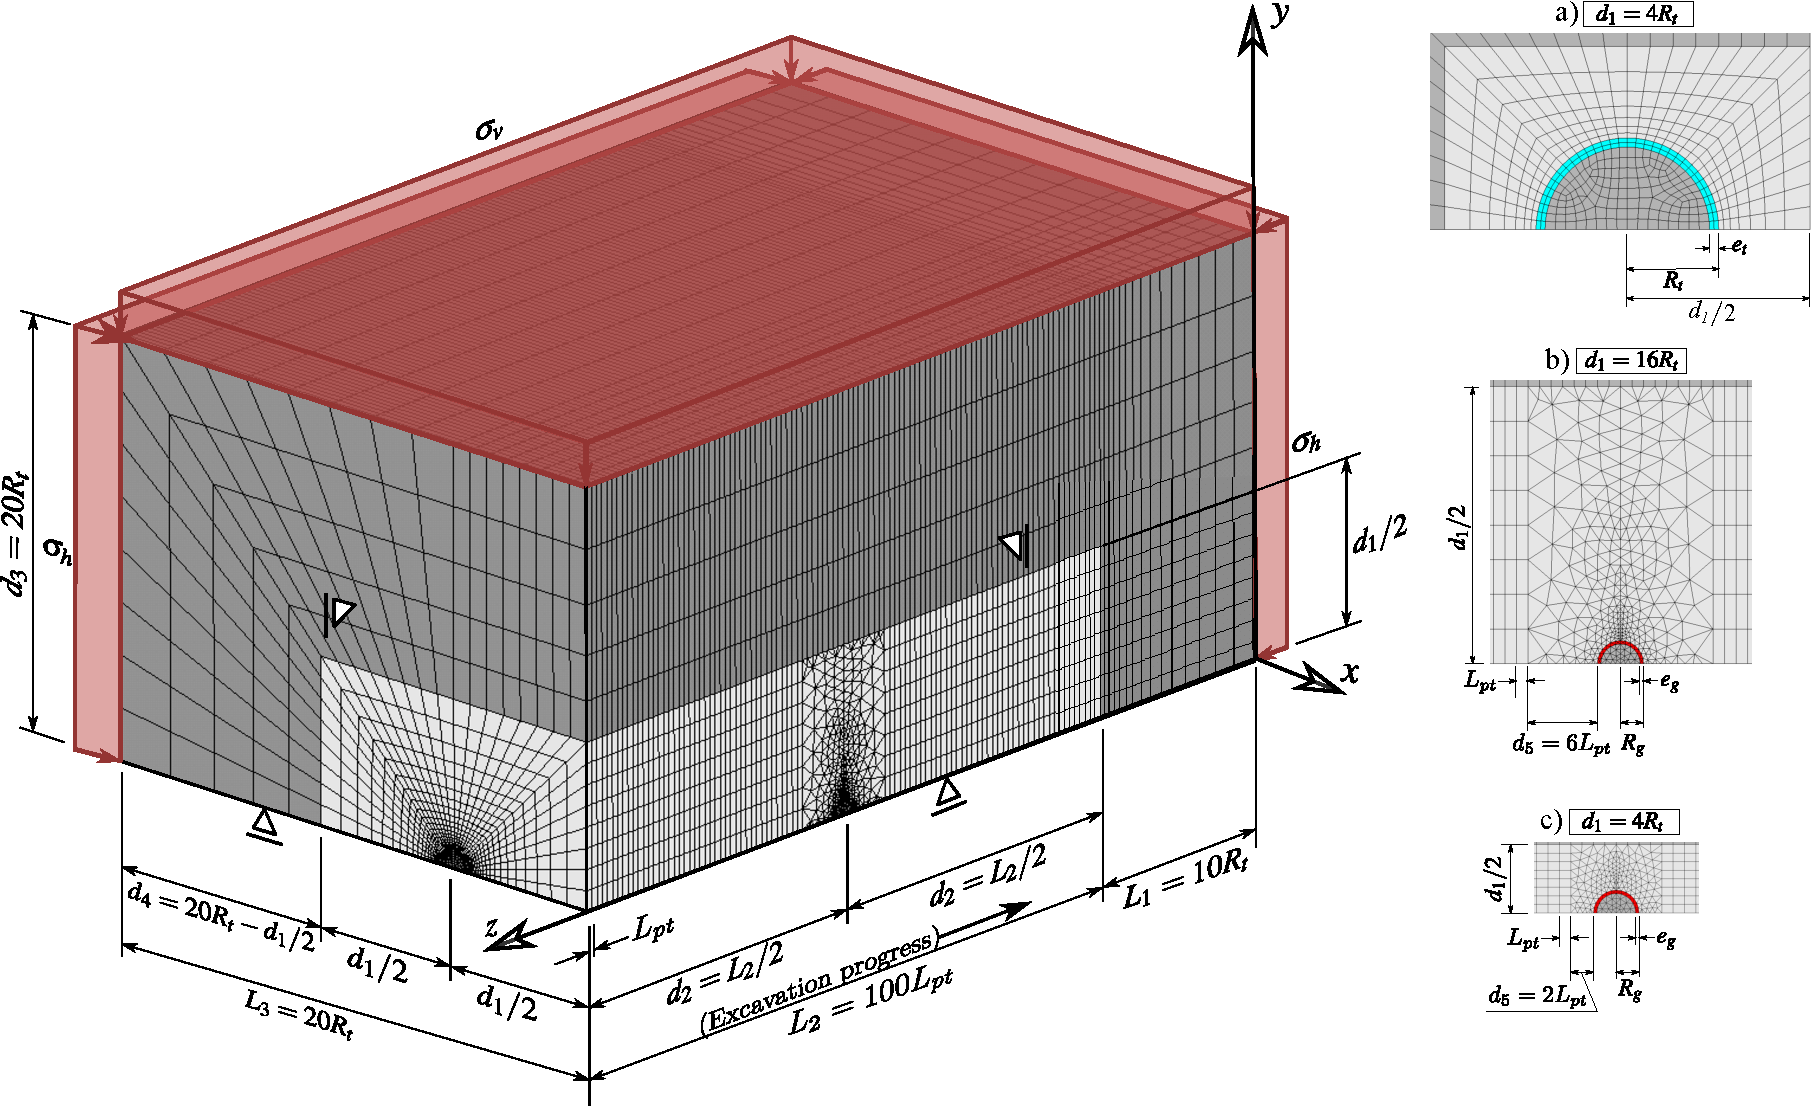
\includegraphics[scale=0.5]{Figures/Mesh1.pdf}
	\caption{Geometry, mesh and boundary conditions of domain and details of a) longitudinal tunnel cross-section for configuration $d_1=4R_t$ and gallery cross-section for configurations b) $d_1=16R_t$ and c) $d_1=4R_t$.}
	\label{Mesh1}
\end{figure}
\FloatBarrier
As mentioned previously, the tunneling process, including the excavation steps and lining installation, is simulated by resorting to the activation-deactivation method shown in the schematic representation in \cref{Diagram of excavations}. Each excavation step is modeled by deactivation of the corresponding elements (the elements stiffness is reduced by a factor $1E8$), whereas installation of elements of lining at a distance $d_{0t}$ from the excavation face (unlined length) is achieved through activation of the corresponding elements by assigning them concrete properties. In this figure, $n_p$ is the total number of excavation steps and $n_{pig}$ represents the number of longitudinal tunnel excavation steps before gallery excavation. After achievement of the $n_{pig}$ excavation steps, the excavation of the gallery is initiated starting from the longitudinal tunnel wall. Referring to the notation of \cref{Diagram of excavations},  $L_{pg}$ is the considered step length for the gallery excavation, and $d_{0g}$ is the unlined length of the gallery. After the gallery excavation is completed, we proceed to further excavation steps of the longitudinal tunnel. The main parameters defining the geometry domain as well as the excavation process and lining installation are summarized in Table~\ref{table1}.

\begin{figure}[h!]
	\centering
	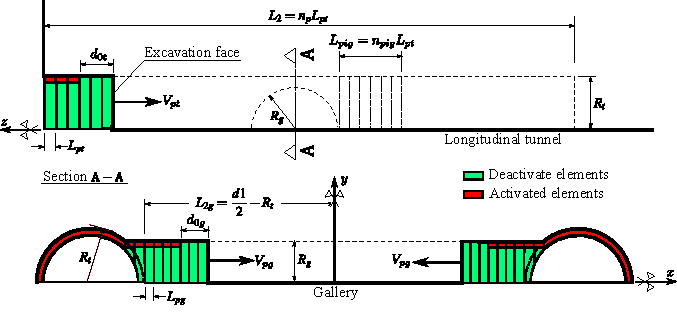
\includegraphics[scale=1.2]{Figures/Diagram of excavations.pdf}
	\caption{Schematic representation of the excavation process.}
	\label{Diagram of excavations}
\end{figure}
\FloatBarrier

\begin{table}
	\caption{Parameters related to the geometry of the domain, excavation and installation of the lining.}
	\label{table1}
	\centering
	%\small
	\renewcommand{\arraystretch}{1.25}
	\begin{tabular}{c c c c}
		\hline
		\multicolumn{1}{c}{PARAMETERS} &
		\multicolumn{1}{c}{SYMBOL} &
		\multicolumn{1}{c}{UNIT} &
		\multicolumn{1}{c}{VALUES} \\
		\hline
		\multicolumn{4}{c}{Longitudinal tunnels} \\
		\hline
		Radius of the longitudinal tunnel & $R_t$ & m & $R_t$ \\
		Thickness of the lining & $e_t$ & m & $0.1R_t$, $0.03R_t$ \\
		Length of the excavation step & $L_{pt}$ & m & $1/3R_t$ \\
		Unlined length & $d_{0t}$ & m & $2L_{pt}$ \\
		\hline
		\multicolumn{4}{c}{Gallery} \\
		\hline
		Radius of the gallery & $R_{g}$ & m & $2/3R_t$ \\
		Thickness of the lining & $e_g$ & m & $e_t$ \\
		Length of the excavation step & $L_{pg}$ & m & $1/3R_g$ \\
		Unlined length & $d_{0g}$ & m & $2L_{pg}$ \\
		Number of steps that starts gallery excavation & $n_{pig}$ & un & $15$ \\
		\hline
		\multicolumn{4}{c}{Rest of domain} \\
		\hline
		Distance between longitudinal tunnel axes & $d_1$ & m & $4R_t, ~16R_t$ \\
		Total length along vertical direction $\ey$ & $d_3$ & m & $20R_t$ \\
		Length of unexcavated region & $L_1$ & m & $10R_t$ \\
		Total excavated length & $L_2$ & m & $100L_{pt}$ \\
		Total length along transversal direction $\ex$ & $L_3$ & m & $20R_t + d_1/2 $ \\
		\hline
	\end{tabular}
	\normalsize
	\\ 
\end{table}
\FloatBarrier
% --------------------------------------------------------------------------
\section{Verification with unlined twin tunnel in elastoplastic medium}\label{sec:format}
% --------------------------------------------------------------------------

In the context of plane strain conditions, \citet{MA2020} developed an approximate analytical solution for the stresses and the plastic zone boundary around deep twin circular tunnels excavated in a homogeneous elastoplastic medium. For the constitutive model, the authors considered perfectly plastic Mohr-Coulomb criterion with associated plastic flow rule. The stress solution for twin tunnels was formulated on the premise that the plastic zone around each tunnel fully encloses the tunnel edge, with the two plastic zones remaining separate and unconnected.

\cref{MA_FIG1} shows the comparison between the 3D F.E. Solution (from a far behind the excavation face) and the analytical solution for plastic zone boundary provided in [\citenum{MA2020}]. For these analysis, $R_t = 1$ m, $d_1/2R_t = 2.5$, rock Young's modulus $E=20$ GPa, Poisson's ratio $\nu = 0.3$ and, friction angle $\phi = 30^\circ$. This analysis shows that finite element modeling produces predictions very similar with those shown in \ref{MA_FIG1}. In addition, the results show that lower values of cohesion $c$ result in larger plastic zones.

\begin{figure}[h!]
	\centering
	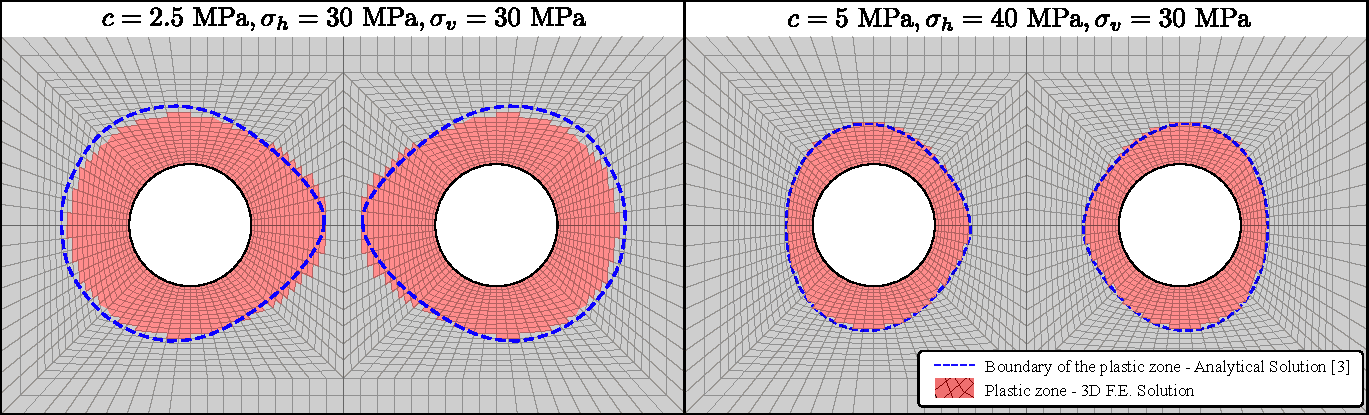
\includegraphics[scale=0.68]{Figures/MA_Comparisions_plastic_zones.pdf}
	\caption{The plastic zone extent obtained from the present F.E. simulations and from the stress solution provided in \citet{MA2020}.}
	\label{MA_FIG1}
\end{figure}
\FloatBarrier

Further comparisons are illustrated in Fig.~\ref{MA_stresspaths}, which shows the radial $\sigma_{rr}$ and orthoradial $\sigma_{\theta \theta}$ stress components along three radial paths defined in polar coordinates by $\theta = 45^\circ$, $90^\circ$, and $135^\circ$. It is important to note that although the finite element simulations use the Drucker-Prager yield surface inscribed within the Mohr-Coulomb surface (as used in the solution by \citet{MA2020}, the numerical predictions closely match the analytical stress solution.

\begin{figure}[h!]
	\centering
	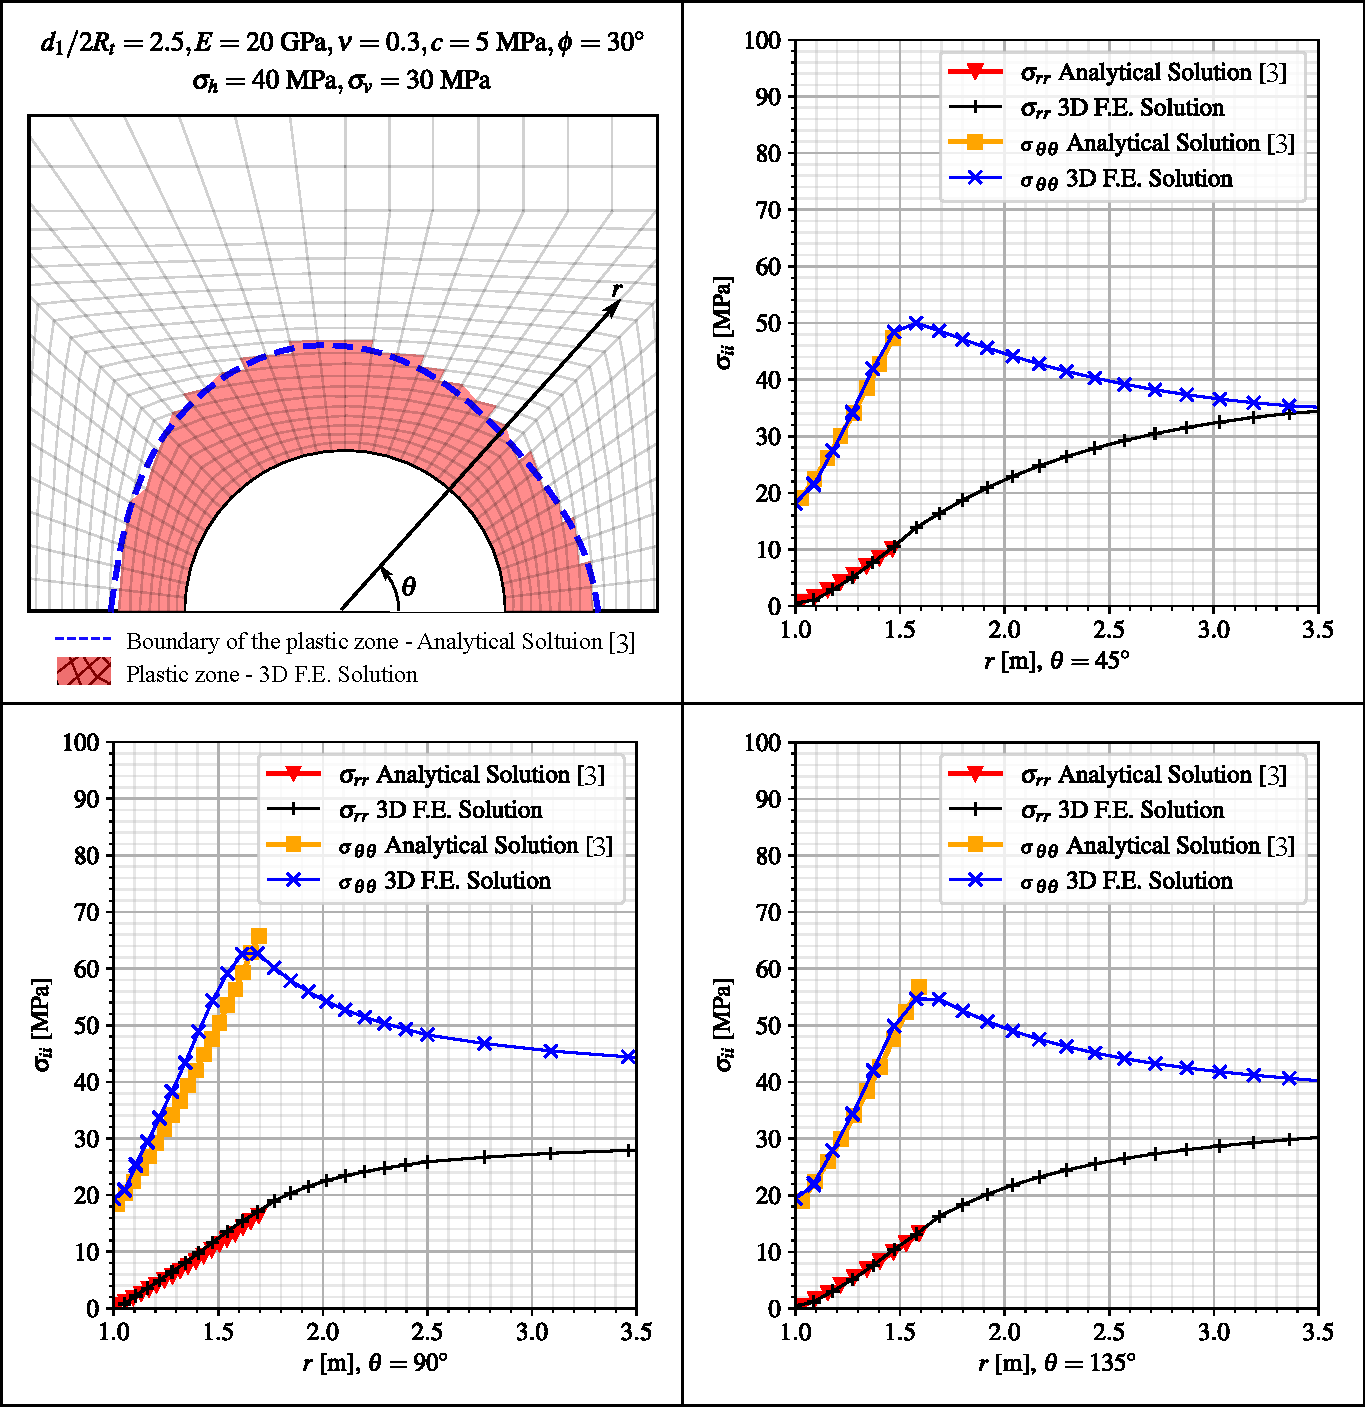
\includegraphics[scale=0.6]{Figures/MA_stresspaths.pdf}
	\caption{Distribution of radial and orthoradial stress components along different radial directions: comparison between numerical and analytical predictions.}.
	\label{MA_stresspaths}
\end{figure}
\FloatBarrier

% --------------------------------------------------------------------------
\section{Numerical Results and Discussion}\label{sec:format}
% --------------------------------------------------------------------------
To develop the analysis, we employed Young's modulus $E = 1500$ MPa, Poisson ratio $\nu = 0.49$, $c = 4\sqrt{3}/2$, $\phi = 0^\circ$ and, isotropic initial stresses $\sigma_v = \sigma_h = 9$ MPa, which correspond to the constitutive parameters and tunneling conditions (450 m depth) in the incompressive clay rock mass in the Paris basin (in Aisne, France), as detailed in  \citet{rousset1988}, \citet{giraud1993} and, \citet{piepi1995}. For the lining, two stiffness values will be considered: $K_c = 969$ MPa and $K_c = 3403$ MPa. Assuming a Young's modulus $E_c = 30303$ MPa and Poisson's ratio $\nu_c = 0.2$, these values corresponds to lining thicknesses $e_t$ of $0.03R_t$ and $0.1R_t$. 

Denoting by $u_y$ the displacement component following the  $y$-axis, \cref{EP_d1_16Ri} and \cref{EP_d1_4Ri} displays the convergence curves $U_B = -u_y(B)/R_t$ that characterize the inward movement at the tunnel roof $B(x=0,y=R_t,z)$ as a function of normalized longitudinal distance to the facing for different conditions: without lining (NL), with elastic lining (EL), with (WG) and without gallary (NG) for $d_1 = 16R_t$ and $d_1 = 4R_t$. In these figures, $U_C$ represents  convergence at $z/R_t = -25$ (far from the effect of the excavation face and gallery), and $U_{D}$ is highlighted at the gallery position $D(x=0, y = R_t, z = L_1+L_2/2)$.

For the single tunnel, the higher stiffness lining (black solid line) reduced convergence by approximately 35\% compared to the unlined scenario (black dashed line). Conversely, the moderately stiff lining (black dotted line) increased convergence by 12\% compared to the higher stiffness lining.

When $d_1 = 16R_t$ (blue and yellow lines), the results of $U_{C}$ are similar to the isolated tunnel (black line). However, with a distance reduced to $d_1 = 4R_t$, the interaction between the tunnels becomes significant. A smaller $d_1$, the higher stiffness lining (yellow and blue solid lines) can restrict convergence by up to 46\% of the unlined (yellow and blue dashed lines) convergence. A moderate stiffness lining (dotted lines) leads to an increase of up to 16\% in convergence compared to the higher stiffness lining (solid lines).

\begin{figure}[h!]
	\centering
	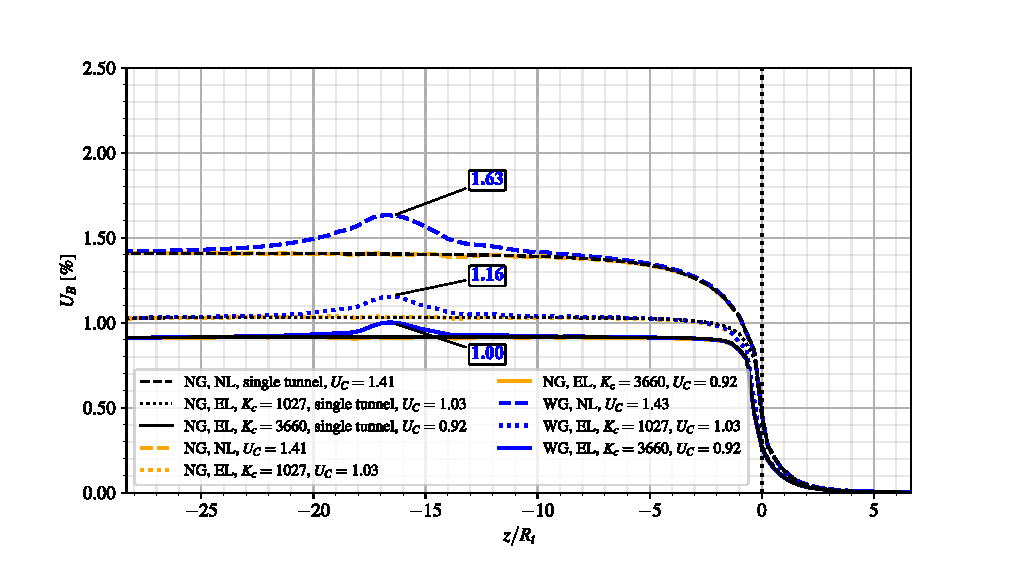
\includegraphics[scale=0.9]{Figures/Convergence Profiles - EP_d1_16Ri_anotate.pdf}
	\caption{Convergence Profiles at the tunnel roof (point B) - for $d_1 = 16R_t$.}.
	\label{EP_d1_16Ri}
\end{figure}
\FloatBarrier
\begin{figure}[h!]
	\centering
	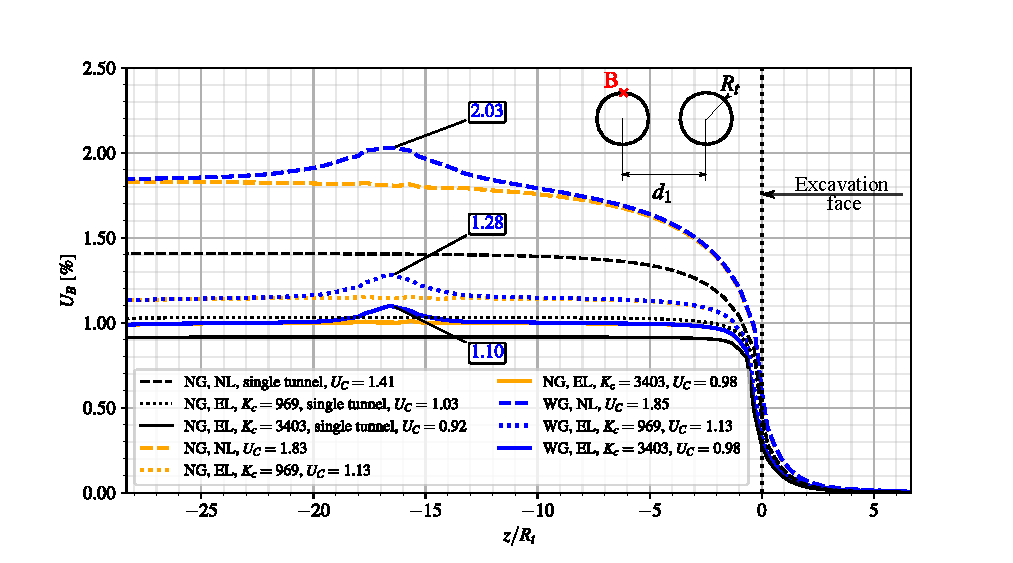
\includegraphics[scale=0.9]{Figures/Convergence Profiles - EP_d1_4Ri_anotate.pdf}
	\caption{Convergence Profiles at the tunnel roof (point B) - for $d_1 = 4R_t$.}.
	\label{EP_d1_4Ri}
\end{figure}
\FloatBarrier

When comparing $U_C$ between twin tunnels with spacings of $16R_t$ and $4R_t$, differences of 6\% with higher stiffness lining (yellow and blue solid lines), 10\% with moderate stiffness lining (yellow and blue dotted lines), and 30\% without lining (yellow and blue dashed lines) are observed. These results show the direct impact of lining stiffness and the distance between twin tunnels on $U_{C}$ convergence.

When analyzing the convergence $U_{D}$ at the point where the gallery meets the longitudinal tunnel, there is an increase of 16\% when using an moderate stiffness lining (blue dotted line) compared to a higher stiffness lining (blue solid line), for both distances $d_1$. However, when analyzing the difference between the $U_{C}$ and $U_{D}$, there is a difference of up to 12\% for the higher stiffness lining (blue solid line to $4R_t$ and $16R_t$) and up to 13\% for the moderate stiffness lining (blue dotted line to $4R_t$ and $16R_t$) for $d_1=4R_t$. In both figures it can be seen that the increase in stiffness reduces the extent of the disturbed region caused by the gallery in the longitudinal tunnel convergence profile. The range decreases from $22.5R_g$ (without lining) to $10.5R_g$ and $7.5R_g$ (with lining). Additionally, the proximity of the tunnel has a minimal impact on the length of this disturbed zone.

% --------------------------------------------------------------------------
\section{Conclusions}\label{sec:conclusion}
% --------------------------------------------------------------------------

Considering the constitutive parameters and tunneling conditions adopted, the analyses show that the lining has a profound impact on the convergence profile of the twin tunnels. It reduces overall convergence by up to 35\% and diminishes the localized convergence of the gallery by approximately a third compared to unlined scenario. In addition, a less rigid lining, approximately 3.5 times less stiff, increases convergence by 12\% and expands the localized effect by 40\% compared to the stiffer lining. Tunnel interaction becomes significant at $4R_t$ however has minimal impact in the range of gallery's localized effect along the longitudinal tunnel.

%-------------------------------------------------------------------------
\vspace{20pt}
\noindent \textbf{Acknowledgements.} The authors are grateful for the financial support provided by CAPES and CNPq.
\vspace{12pt}

%--------------------------------------------------------------------------
\noindent \textbf{Authorship statement.} The authors hereby confirm that they are the sole liable persons responsible for the authorship of this work, and that all material that has been herein included as part of the present paper is either the property (and authorship) of the authors, or has the permission of the owners to be included here. 

\bibliography{bibliography}

\end{document}
% --------------------------------------------------------------------------
